\section{第一类曲线积分}

本节讨论第一类曲面积分。
所谓“第一类曲面积分”是数量值函数对曲面的积分。

本节要点:
\begin{itemize}
    \item 掌握第一类曲面积分的概念;
    \item 掌握第一类曲面积分的计算,重点掌握曲面微元的计算。
\end{itemize}

%============================================================
\subsection{第一类曲面积分的概念}

\begin{definition}[第一类曲面积分]
若三维空间中有曲面$S$,$f\left( \boldsymbol{p} \right) ,\boldsymbol{p}\in \mathbb{R} ^3$为定义在该空间上的三元数量值函数,若下式极限存在,则称极限值为{\bf $f\left( \boldsymbol{p} \right) $在$S$上积分称为第一类曲面积分},记为$\iint_S{f\left( \boldsymbol{p} \right) ds}$,即:
\[
\iint\limits_S{f\left( \boldsymbol{p} \right) ds}:=\underset{\lambda \rightarrow 0}{\lim}\sum_{i=1}^n{\left[ f\left( \xi _i,\eta _i,\zeta _i \right) \cdot \Delta s_i \right]}
\]
其中:
\begin{itemize}
    \item $f\left( \boldsymbol{p} \right) $:{\bf 被积函数};
    \item $ds$:{\bf 曲面微元};
    \item $S$:{\bf 积分曲面}。
\end{itemize}
\end{definition}

\begin{tcolorbox}
实际定义参考“教材\cite{book1}”,这里是一个简写,总体来讲就是将曲面分片,每片上取一个值和这一小片面积乘积$f\left( \xi _i,\eta _i,\zeta _i \right) \cdot \Delta s_i$,如果和式有极限,则成为$f\left( \boldsymbol{p} \right) $在$S$上有第一类曲面积分。
大致思路和一元函数积分一样。
\end{tcolorbox}

简单说明曲面微元$ds$和{\it xOy}平面投影微元$d\sigma $的关系,这是求解第一类曲面积分的关键。
如果曲面在被积范围内可微,则某点处的曲面微元$ds$与该点处的切面微元$dA$的面积相等。
若曲面由$z=z\left( x,y \right) $显式给出,则切面的法向量为$\boldsymbol{n}=\left( -z_x\,\,-z_y\,\,1 \right) ^T$。
假设法向量和{\it z}轴成角$\theta $,则有:
\[
\cos \theta =\frac{1}{\sqrt{\left( z_x \right) ^2+\left( z_y \right) ^2+1}}
\]
则切面微元$dA$和{\it xOy}平面投影微元$d\sigma $有关系:
\[
d\sigma =\cos \theta \cdot dA=\frac{1}{\sqrt{\left( z_x \right) ^2+\left( z_y \right) ^2+1}}\cdot dA
\]
可得曲面微元$ds$和{\it xOy}平面投影微元$d\sigma $的关系:
\[
ds=\sqrt{\left( z_x \right) ^2+\left( z_y \right) ^2+1}\cdot d\sigma =\sqrt{\left( z_x \right) ^2+\left( z_y \right) ^2+1}\cdot dxdy
\]

\begin{figure}[h]
\centering
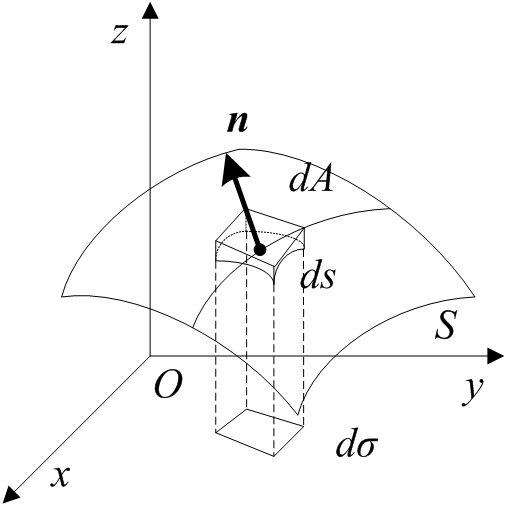
\includegraphics[height=4cm]{10.1.png}
\end{figure}

%============================================================
\subsection{第一类曲面积分的计算}

\begin{theorem}[第一类曲面积分的计算公式]
若$f\left( \boldsymbol{p} \right) $在曲面$S$上连续,$z=z\left( x,y \right) $在$S$上具有一阶连续偏导,则第一类曲面积分的计算公式有:
\begin{align*}
&\iint\limits_S{f\left( \boldsymbol{p} \right) ds}=\iint\limits_D{\left[ f\left( x,y,z\left( x,y \right) \right) \cdot \sqrt{\left( z_x \right) ^2+\left( z_y \right) ^2+1} \right] dxdy} \\
&S=\left\{ \left( x,y,z \right) \middle| x_1\leqslant x\leqslant x_2,y_1\left( x \right) \leqslant y\leqslant y_2\left( x \right) ,z=z\left( x,y \right) \right\} \\
&D=\left\{ \left( x,y \right) \middle| x_1\leqslant x\leqslant x_2,y_1\left( x \right) \leqslant y\leqslant y_2\left( x \right) \right\}
\end{align*}
\end{theorem}

第一类曲面积分的计算关键在于理解曲面微元和投影微元的关系:
\[
ds=\sqrt{\left( z_x \right) ^2+\left( z_y \right) ^2+1}\cdot d\sigma =\sqrt{\left( z_x \right) ^2+\left( z_y \right) ^2+1}\cdot dxdy
\]
通过这个关系,将第一类曲面积分化为二重积分。




